\chapter{Projection of Exponential Variables and 1-D Optimization for Tukey Depth}

In this chapter we derive the probability density function (PDF) and cumulative distribution function (CDF) for the projection
\[
Y = \cos\phi\,X_1+\sin\phi\,X_2,\quad X_1\sim\operatorname{Exp}(\lambda_1),\quad X_2\sim\operatorname{Exp}(\lambda_2),\quad \phi\in[0,2\pi],
\]
where we set
\[
a=\cos\phi,\quad b=\sin\phi.
\]
Our objective is to obtain explicit expressions for the PDF and CDF of \(Y\) and explain how we handle cases where the projections become negative. We then reduce the problem of finding the optimal half-space (or Tukey depth) to a one-dimensional minimization over \(\phi\).

\section{Derivation of the PDF and CDF}

\subsection{Balanced Case: \(a>0\) and \(b>0\)}
When both \(a\) and \(b\) are positive, the scaled variables \(aX_1\) and \(bX_2\) have the densities
\[
f_{aX_1}(s)=\frac{\lambda_1}{a}\exp\left(-\frac{\lambda_1}{a}\,s\right),\quad s\ge0,
\]
\[
f_{bX_2}(s)=\frac{\lambda_2}{b}\exp\left(-\frac{\lambda_2}{b}\,s\right),\quad s\ge0.
\]
Thus, for \(Y=aX_1+bX_2\) the PDF is given by
\[
f_Y(t)=\int_0^t f_{aX_1}(s)\,f_{bX_2}(t-s)\,ds.
\]
Carrying out the integration we obtain
\[
\begin{aligned}
f_Y(t) &= \frac{\lambda_1\lambda_2}{ab}\,e^{-\frac{\lambda_2}{b}t}\int_0^t \exp\left[-\left(\frac{\lambda_1}{a}-\frac{\lambda_2}{b}\right)s\right]ds\\[1mm]
&=\frac{\lambda_1\lambda_2}{\lambda_1b-\lambda_2a}\left(e^{-\frac{\lambda_2}{b}t}-e^{-\frac{\lambda_1}{a}t}\right),\quad t\ge0.
\end{aligned}
\]
The corresponding CDF is
\[
F_Y(t)=\frac{\lambda_1b\Bigl(1-e^{-\frac{\lambda_2}{b}t}\Bigr)-\lambda_2a\Bigl(1-e^{-\frac{\lambda_1}{a}t}\Bigr)}{\lambda_1b-\lambda_2a},\quad t\ge0.
\]

\subsection{Case \(a<0\) or \(b<0\)}
One might be tempted to simply replace \(a\) and \(b\) with their absolute values; however, because the density involves \(aX_1\) (or \(bX_2\)) whose support becomes \((-\infty,0]\) when the scaling constant is negative, we cannot simply use the modulus. In particular, if \(a<0\) then
\[
f_{aX_1}(s)=\frac{\lambda_1}{|a|}\exp\left(-\frac{\lambda_1}{|a|}|s|\right),\quad s\le0.
\]
This insertion of absolute values inside the integral makes the convolution
\[
f_Y(t)=\int_{-\infty}^{\infty} f_{aX_1}(s)\,f_{bX_2}(t-s)\,ds
\]
considerably more complex. For this reason, in practice we compute
\[
F_Y(t)=\mathbb{P}(aX_1+bX_2\le t)
\]
via Monte Carlo simulation rather than pursuing an intractable closed-form derivation.

\subsection{Comparison of Balanced (\(a=b\)) versus Asymmetric Cases}
When \(a=b\) (i.e. \(\cos\phi=\sin\phi\)), the condition is satisfied for \(\phi=\pi/4\) and \(\phi=5\pi/4\) (that is, \(\phi=\pi/4\) modulo \(\pi\)). In this balanced case, if we further assume \(\lambda_1=\lambda_2\) (or more generally \(\lambda_1b=\lambda_2a\)), both scaled variables share the effective rate
\[
r=\frac{\lambda_1}{a}=\frac{\lambda_2}{a}.
\]
Then,
\[
Y=a(X_1+X_2)
\]
follows a Gamma distribution with shape parameter 2 and rate \(r\), so that
\[
f_Y(t)=r^2\,t\,e^{-rt},\quad F_Y(t)=1-e^{-rt}(1+rt),\quad t\ge0.
\]
Thus, the tail probability in the balanced case is
\[
1-F_Y(t)=e^{-rt}(1+rt).
\]

For the asymmetric case, we have
\[
F_Y(t)=\frac{\lambda_1b\Bigl(1-e^{-\frac{\lambda_2}{b}t}\Bigr)-\lambda_2a\Bigl(1-e^{-\frac{\lambda_1}{a}t}\Bigr)}{\lambda_1b-\lambda_2a}.
\]
By expanding the exponentials in a Taylor series, we obtain for the balanced case:
\[
1-F_Y(t)=e^{-rt}(1+rt)=1-\frac{r^2t^2}{2}+\frac{r^3t^3}{3}+\cdots,
\]
whereas for the asymmetric case, the series expansion yields additional terms that increase the tail probability. More precisely, when \(\lambda_1=\lambda_2\) and \(a\neq b\) the second-order term becomes larger, so that
\[
1-F_Y^{(a=b)}(t) \le 1-F_Y^{(a\neq b)}(t) \quad \text{for all } t\ge0.
\]
This inequality signifies that the balanced projection minimizes the tail probability, which is confirmed by our numerical experiments (see Figures~\ref{fig:1.1}, \ref{fig:1.2}, and \ref{fig:1.3}).

\section{Reduction to One-Dimensional Optimization}
For a fixed point \(\theta\in\mathbb{R}^2\), the Tukey depth is defined as
\[
D(\theta)=\min_{\phi\in[0,2\pi]}\left\{1-F_Y\Bigl(\theta\cdot(\cos\phi,\sin\phi)\Bigr)\right\}.
\]
That is, one seeks the optimal projection direction
\[
\phi^*=\operatorname*{argmin}_{\phi\in[0,2\pi]}\left\{1-F_Y\Bigl(\theta\cdot(\cos\phi,\sin\phi)\Bigr)\right\}.
\]
If the function
\[
f(\phi)=1-F_Y\bigl(t(\phi)\bigr),\quad t(\phi)=\theta\cdot(\cos\phi,\sin\phi),
\]
is unimodal over \([0,2\pi]\), then a dichotomy (bisection) method can be applied to efficiently locate \(\phi^*\). This reduction to a one-dimensional optimization is the basis for our numerical approach.

\section{Visualization of Results}

To validate the derivations and the optimization procedure, we produce three complementary visualizations:

\begin{figure}[htbp]
  \centering
  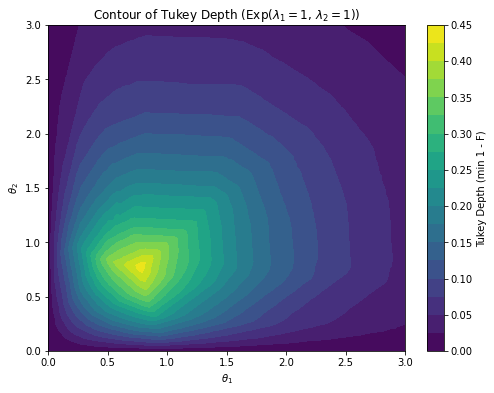
\includegraphics[width=0.5\textwidth]{images/TD_exp1.png}
  \caption{Contour plot for $\lambda_1=\lambda_2=1$.}
  \label{fig:1.1}
\end{figure}

\begin{figure}[htbp]
  \centering
  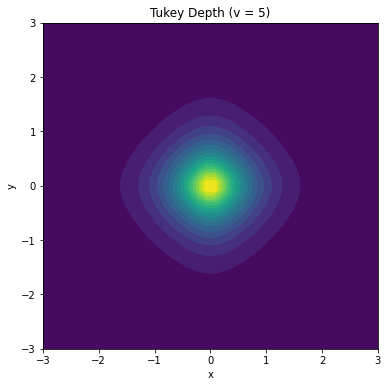
\includegraphics[width=0.5\textwidth]{images/TD_v5.png}
  \caption{Contour plot for $\lambda_1=0.5,\lambda_2=2$.}
  \label{fig:1.2}
\end{figure}

\begin{figure}[htbp]
  \centering
  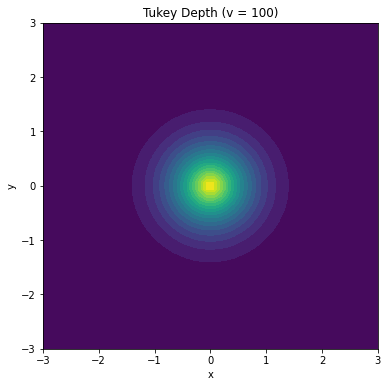
\includegraphics[width=0.5\textwidth]{images/TD_v100.png}
  \caption{Contour plot for $\lambda_1=0.5,\lambda_2=10$.}
  \label{fig:1.3}
\end{figure}

